\documentclass{report}


\usepackage{amsmath} % Better matrix environment
\usepackage{amssymb}
\usepackage[inline]{enumitem} % inline numbering and resume numbering
\usepackage{etoolbox} % If conditions
\usepackage{graphicx}
\usepackage{listings} % for code
\usepackage{nth}
\usepackage{hyperref}
\usepackage{cleveref} % Must be loaded after hyperref
\usepackage{caption}
\usepackage{pgfplotstable}
\pgfplotsset{compat=1.10}
\usepackage{subcaption}
\usepackage{svg}
\usepackage{tikz}
\usepackage{tikz-qtree,tikz-qtree-compat} % Trees
\usepackage{url}
\usepackage{xkeyval}

\pdfoptionpdfminorversion=5

% Squiggly lines
\usetikzlibrary{decorations.pathmorphing}


% Node shapes
\usetikzlibrary{shapes,decorations}

% Coordinate calculation
\usetikzlibrary{calc}

% For charts
\usetikzlibrary{patterns}

\newcommand{\VertexSet}{V}
\newcommand{\CellSet}{C}

\newcommand{\Visited}{V_{visited}}

% Cardinality of
\newcommand{\card}[1]{\left\vert{#1}\right\vert}

% powerset of
\newcommand{\powerset}[1]{\mathcal P \left({#1}\right)}



% Line that can go anywhere, structured region or outside
\tikzset{%
    anywhere/.style={
		decorate,
		decoration={
		    snake,
		    segment length=4,
		    amplitude=.9,post=lineto,
		    post length=2pt
		}
	}
}

% Line that can only go outside the structured region
\tikzset{outside/.style={dotted}}


% Ellipsis
\tikzset{ellipsis/.style={loosely dotted}}



\begin{document}

\chapter{Introduction}
Scientific computing is a large research branch touching on various areas in the scientific community as well as in various industries. An integral part of it is concerned with algorithms and techniques which operate on a mesh representation of a model, typically modelling physical phenomena such as the motion of fluids. SEE
% [Flow simulation and high performance computing, 1996a T. Tezduyar, http://www.tafsm.org/PUB_PRE/jALL/j63-CM96.pdf]
. SEE
% [http://www.sv.vt.edu/classes/MSE2094_NoteBook/97ClassProj/num/widas/history.html]
for a good introduction on finite element analysis.


Various methods of representing meshes exist, including X, Y, and Z
% [http://en.wikipedia.org/wiki/Polygon_mesh#Representations]
. Representations typically rely on encoding some form of explicitly-defined mapping between mesh elements. This can be represented straightforwardly as a flat array, with the array indices representing elements in the source set, and each value being one or more values representing one or more elements in the destination/target set. We focus our attention to the case where the number of target elements mapped to from each source element is constant. Such a map is known as a constant-arity map.

Consider for instance a quadrilateral mesh with two element sets \texttt{C} and \texttt{V}, representing the set of cells and vertices, respectively.
We can define a dat of coordinates, which associates the set each vertex $v \in V$ with a coordinate pair $(x_v, y_v)$, representing its position in 2D space.

We can then define an adjacency map (of constant arity 4) from cells to vertices:

\texttt{$C \rightarrow Node^4$}

Now consider an operation over this mesh, which performs a computation for each cell $c \in C$ as a function of its adjacent nodes ${n | n \in Map[c]}$, for instance computing the area of the cell. In particular consider the chain of memory access indirections and the resulting memory access patterns:

%
%             |   |             |   |
%             |   |  /----n3--->|   | -> (x_1, y_1)
%             |   | /           |   |
% cell_id ->  |   |/------n1--->|   | -> (x_4, y_4)
%             |   |\            |   |
%             |   | \-----n4--->|   | -> (x_5, y_5)
%             |   |  \          |   |
%             |   |   \---n2--->|   | -> (x_12, y_12)
%             |   |             |   |
%             |   |             |   |
%             |   |             |   |
%           cell2nodes         node2coordinate

Notice that proximate (or indded adjacent) nodes in the mesh need not exhibit a uniform memory access pattern. This is detrimental to performance for various reasons.
1. They do not exhibit spatial locality, a property which most modern CPU caches bank on to attain higher performance in IO bound applications, which may manifest through decisions regarding cache replacement strategies or data pre-fetching.
2. Looking up addresses, as opposed to computing them directly, will typically prohibit or limit the scope of compiler-performed optimizations, not least vectorizations.

Numerous strategies have been devoted to deal with this problem, notably applying a space filling curve to obtain a more favourable numbering, with closer elements tending to have closer numberings. While the space filling curve most certainly improves cache locality, it does not make use more obvious structure that may exist. A mesh that is irregular and unstructured on the whole may contain subregions of high regularity and uniform structure, whose regularity/uniformity may be locally exploitable in a more direct manner, for potentially higher gain!


We present Crystal mesh, a group of algorithms for \emph{extracting} regions of regularity in a mesh, reorganizing the mesh to \emph{expose} said structure in order to enable efficient \emph{exploitation}.
In particular, we present and evaluate an implementation for extracting and exposing structure in quadrilateral meshes on various examples, and evaluate a 33\% performance improvement achieved by exploiting the structure on the airfoil computation.


\chapter{Background}
\section{The mathematical mesh model}

Meshes often model physical objects and phenomena. This is typically achieved through the discretization of a continuous model, such as the surface or volume of an object, in order to approximate its physical properties to a desired degree of precision.
\par

The mesh model consists of a hierarchy of elements, which may include a subset the following:
\begin{itemize}
\item Polyhedra such as cubes or tetrahedrons
\item Polygons \emph{(also referred to as cells or faces)} such as triangles and quadrilaterals
\item Edges
\item Vertices \emph{(also referred to as nodes)}
\end{itemize}

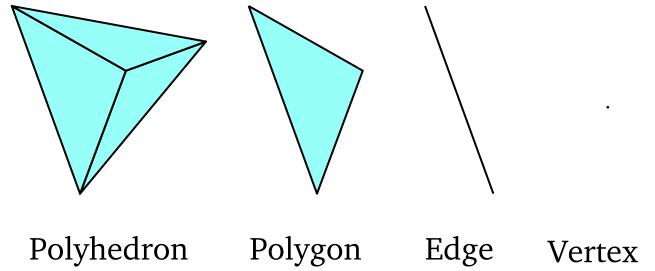
\includegraphics[scale=0.5]{images/background/mesh-elements.pdf}

Each element in the above hierarchy is built-up from those below it. Thus, a polyhedron is assimilated by a set of polygons, a polygon is composed by a set of edges, and an edge joins two vertices.


\subsection{Geometry vs topology}
There is a key distinction to make between the geometric and topological properties of a mesh.

Since meshes model a physical reality, the elements of a mesh may be spatially embedded: vertices are associated with points in space, and edges are formed as segments joining their two vertices. This affects \emph{geometric} properties of the mesh, such as its surface area or volume.

On the other hand, the hierarchy of elements described above induces a mesh topology. This describes the connectedness of the mesh, that is to say how elements relate to one another. For instance, we may describe two vertices sharing an edge as \emph{adjacent}, or two cells being \emph{incident} on an edge.
\par
In this work we concern ourselves solely with the topological structure of meshes, treating its geometry as arbitrary data that is associated with its respective elements (the position of a vertex for instance). Figure~\ref{fig:same-topology} illustrates the difference between the two concepts.

\begin{figure}
    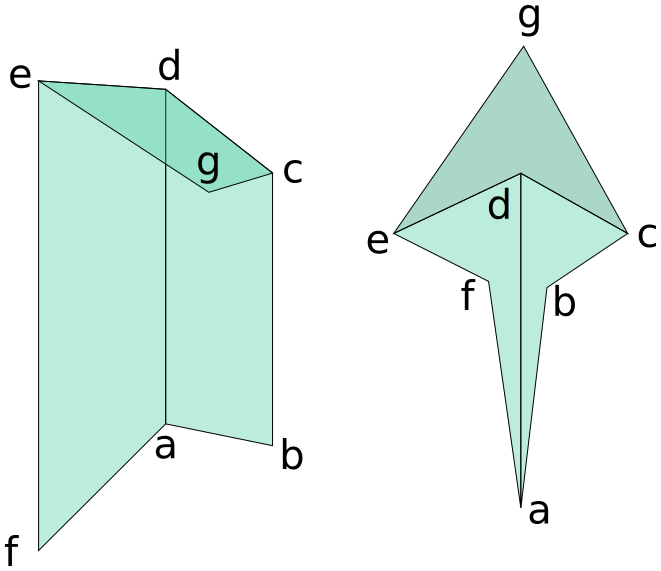
\includegraphics[scale=0.5]{images/background/same-topology.pdf}
    \caption{Despite having completely different geometric shapes and properties, the two meshes are topologically equivalent. The labels indicate corresponding vertices.}
    \label{fig:same-topology}
\end{figure}




\subsection{Manifold meshes}
A mesh is a manifold if the following properties hold:
\begin{enumerate}
\item All edges are adjacent to either one or two faces.

\item All faces meeting at a given vertex must form either an open or a closed fan around that vertex (Figure~\ref{fig:open-closed-fans}).
\end{enumerate}

% Open and closed fans
\begin{figure}
    \sidebyside
        {\includegraphics[scale=0.2]{images/background/closed-fan.pdf}
        \caption{A closed fan}}
        {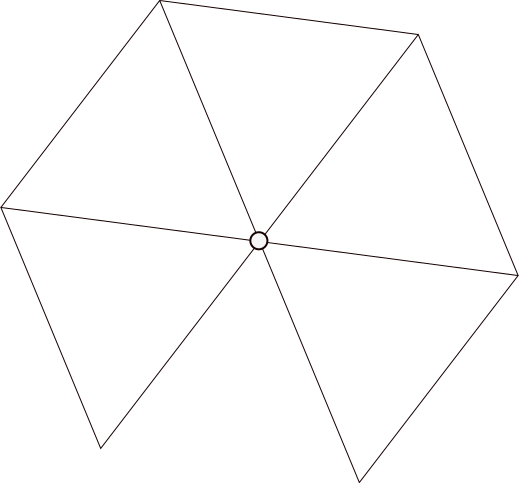
\includegraphics[scale=0.2]{images/background/open-fan.pdf}
        \caption{An open fan}}
    \caption{}
    \label{fig:open-closed-fans}
\end{figure}

Figure~\ref{fig:non-manifolds} demonstrates examples of non-manifold meshes.

% Non-manifolds
\begin{figure}
    \sidebysidefour
    {\includegraphics[scale=0.2]{images/background/bad-fan.pdf}
        \caption{Faces incident on a vertex which do not form a continuous fan}}
    {\includegraphics[scale=0.2]{images/background/bad-fan2.pdf}
        \caption{An extra face that breaks off from the otherwise closed fan}}
    {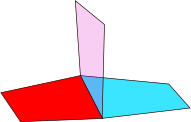
\includegraphics[scale=0.8]{images/background/bad-multi-edge.pdf}
        \caption{More than two faces incident on a single edge}}
    {\includegraphics[scale=0.8]{images/background/bad-no-edge.pdf}
        \caption{An edge with no incident faces}}

    \caption{Examples of non-manifold meshes.}
    \label{fig:non-manifolds}
\end{figure}

In this work we consider manifold meshes exclusively, and future mentions of `mesh' shall implicitly refer to manifold meshes.




\section{The mesh data structure}

We describe how a mesh model is manifest at the data structure level. There are three general component types can be identified:
\begin{itemize}
\item Entity sets
\item Associative data
\item Relations between two entity sets
\end{itemize}

In the following sections, the examples shall refer to the mesh depicted in figure~\ref{fig:example-mesh}.

\begin{figure}
    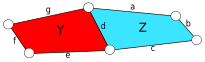
\includegraphics[scale=2]{images/background/mesh-data-structure.pdf}
    \caption{Example mesh with labelled elements.}
    \label{fig:example-mesh}
\end{figure}


\subsection{Entity sets}
Each set represents a certain type of entity in the mesh, such as vertices or cells. Each element in a set is associated with a unique identifier. Integers are a common choice as an identifier for a couple of reasons:
\begin{itemize}
\item They need not be enumerated explicitly. All we need is the set cardinality and a starting index.
\item They are convenient for direct-indexed array accesses, as well as for more general indexing methods.
\end{itemize}

See figure~\ref{fig:entity-sets} for examples.

\begin{figure}
    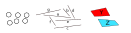
\includegraphics[scale=4]{images/background/entity-sets.pdf}
    \caption{The entity sets of the mesh in figure~\ref{fig:example-mesh}. These are (from left to right) the vertices, edges, and cells.}
    \label{fig:entity-sets}
\end{figure}


\subsection{Associative data}
Arbitrary data which is associated with elements of a particular entity set. For instance, spatial coordinates associated with each vertex. A typical representation is a flat array indexed by element identifier.
This is the data over which we perform our computations and ultimately care about. Everything else is incidental.

See figure~\ref{fig:associative-data} for an example.

\begin{figure}
    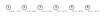
\includegraphics[scale=4]{images/background/associative-data.pdf}
    \caption{Coordinate data associated with the vertices of the mesh in figure~\ref{fig:example-mesh}.}
    \label{fig:associative-data}
\end{figure}


\subsection{Relation maps between two entity sets}
Entity sets may have relations defined between them, a mapping from an element in a source set to one or more corresponding elements in the destination set. For instance, we may have an adjacency relation from the vertex set to itself, or an inclusion relation from the cell set to the vertex set.
In a general unstructured mesh these relations must be explicitly stored, typically as an array indexed by the source element's identifier.

See figure~\ref{fig:relation} for an example.

\begin{figure}
    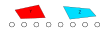
\includegraphics[scale=4]{images/background/relation.pdf}
    \caption{Inclusion relation from cells to vertices, as depicted in the mesh of figure~\ref{fig:example-mesh}.}
    \label{fig:relation}
\end{figure}




\section{The mesh core-computation contract}
Given a mesh model and its underlying representation, computation logic provided by an external user is to be executed. We refer to this as the \emph{core-computation}; this is to disambiguate it from other incidental processing, such as structure detection.
Our contract to the user is described in what follows.

\subsection{Given: entity set}
We are given an entity set over which to operate, for example the set of edges or the set of cells. The core-computation consists of executing a computation for each element of this set. This is analogous to the \emph{map} phase of the MapReduce programming model\footnote{REFERENCE}, though we restrict our usage of the term \emph{map} to refer to relation maps.

\subsection{Given: relation-map tree}
We are given a tree structure defining which relation maps to use and how to access them. This is best explained through an example, illustrated in figure~\ref{fig:relation-tree}.


\begin{figure}
    %% Key icon
    \newcommand{\keyicon}{
\includegraphics[width=6pt]{images/background/key.pdf}}

    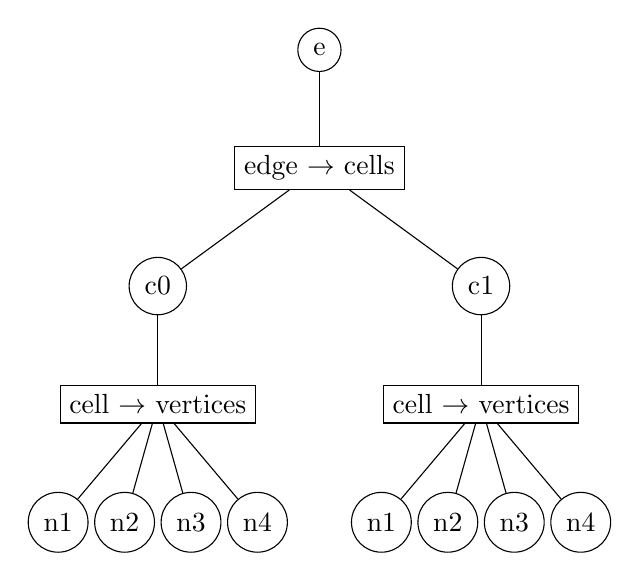
\begin{tikzpicture}[every tree node/.style={draw,circle},
        level distance=1.5cm,
        edge from parent path={(\tikzparentnode) -- (\tikzchildnode)}]

    \tikzset{level 2/.style={sibling distance=0.8cm}}

    \Tree
    [.{e}
        \edge node[auto=right] {\keyicon};
        [.\node[rectangle] {edge $\rightarrow$ cells};
            [.{c0}
                \edge node[auto=right] {\keyicon};
                [.\node[rectangle] {cell $\rightarrow$ vertices};
                    [.n1 ]
                    [.n2 ]
                    [.n3 ]
                    [.n4 ]
                ]
            ]
            [.{c1}
                \edge node[auto=right] {\keyicon};
                [.\node[rectangle] {cell $\rightarrow$ vertices};
                    [.n1 ]
                    [.n2 ]
                    [.n3 ]
                    [.n4 ]
                ]
            ]
        ]
    ]
    \end{tikzpicture}
    \caption{EXPLANATION}
    \label{fig:relation-tree}
\end{figure}





% \item The entity set over which to operate.
% \item Any relation maps to follow, and the variables by which they are indexed. Indexing variables may include the current iteration element, as well as the targets got by following another map.
% In general this may involve complex chains of maps, though only up to to two levels of indirection are used in practice.
% \item A kernel function which is to be applied to each element in the given entity set.
% \end{itemize}

A \emph{kernel function} specifying the computation logic is given. This kernel function is associated with a particular entity set.

The execution contract

When performing some computation over a mesh, the data access pattern followed is typically as follows:
\begin{enumerate}
\item Iterate over the elements of an entity set, in no particular order.
\item For each element iterated over, gather any handles to associated elements (the indices of adjacent elements, say). This may involve handles obtained through a chain of set relationship maps.
\item Access the associative data using the gathered handles.
\end{enumerate}


 The computation is often specified as a \emph{kernel function} operating a particular entity set



\chapter{Related works}
% \section{Structure is beneficial}



% - How do quad meshes with subregions of structure come about
% - Are they seen often


\section{Structure detection and extraction}


% Fast Neighborhood Search on Polygonal Meshes
% http://www.inf.ethz.ch/personal/dpanozzo/papers/EGIT11-RocDeGPanPup.pdf
% Dude et al tackle the specific problem of neighborhood search by defining a spatial index, a hierarchy of clusters of vertices. Their method yields an approximation, ours is exact, with the mesh model left completely unaltered. However, we can learn a few things.

% The problem of indirections and its derivatives (non-contiguous memory access and its impact on cache hierarchy) is cited/highlighted as a key motivation in basing their mesh data structure on a geometric model, i.e. the spatial index. We undertake the opposite approach, viewing geometric data as mere associative data attached to a topological mesh model.

Adapting the mesh model to use a structured representation for the benefit of the relevant application domain is (not new) / (fairly prevalent).
Rocca et al.~\cite{rocca2011fast} address the particular problem of neighbourhood search: finding the set of vertices within a certain distance from a given vertex. They define a spatial index, a hierarchy of vertex clusters, that yields good approximations to neighbourhood search queries.

The problem of memory access indirections, associated with representing the mesh topology, is cited as a key motivation for basing their mesh data structure (the aforementioned spatial index) on a geometric model which does not require storing topological information. This is in sharp contrast to our approach of transforming the mesh topology representation, and treating the mesh geometry as arbitrary associative data.



% Motorcycle Graphs: Canonical Quad Mesh Partitioning
% http://www.ics.uci.edu/~goodrich/pubs/geomproc.pdf
% Whilst the motivations are different (mesh compression AND mesh isomorphism) the approach is similar:
% ``The simplest quadrilateral meshes are structured meshes, in which connections between quadrilaterals form a regular grid, but in complicated domains it may be necessary to use semi-regular meshes in which this structure is interrupted by a small number of extraordinary vertices that do not have degree four. We study how to partition a semi-regular mesh into a small number of structured submeshes.''


% ``To ensure that isomorphisms will always be found when they exist, our partition must be canonical: the same mesh must always generate the same partition. The partitioning algorithm we describe has this property.''
% We do not care about this property per se. There may be multiple optimal solutions for structure detection, for example.


% ``Additionally, these techniques may apply to areas beyond graphics such as scientific computation. Code for the finite element method can be greatly streamlined when applied to structured quadrilateral meshes. By partitioning unstructured meshes into structured submeshes, it should be possible to achieve similar speedups for semi-regular meshes.''

Eppstein et al.~\cite{eppstein2008motorcycle} describe a method for partitioning quadrilateral meshes into structured regions using the \emph{motorcycle graph} construction, whose inspiration came from the 1982 movie Tron. The algorithm works by placing particles on each \emph{extraordinary} vertex\footnote{\label{footnote:extraordinary-vertices} This is in contrast to an \emph{ordinary} vertex, which the authors define as ``a non-boundary vertex incident with four edges or a boundary vertex incident with at most three edges.''} in the mesh, and advancing them along edges until they collide. The enclosed regions formed by the paths represent structured regions.

Whilst the motivations are different, with the emphasis on applications in mesh compression and detecting mesh isomorphisms, the approach may be applicable to the scientific computation domain. Indeed, the authors state this explicitly:
\begin{quote}
These techniques may apply to areas beyond graphics such as scientific computation. Code for the finite element method can be greatly streamlined when applied to structured quadrilateral meshes. By partitioning unstructured meshes into structured submeshes, it should be possible to achieve similar speedups for semi-regular meshes.
\end{quote}

We note, however, that the method makes a stronger assumption about the mesh, in that its ``structure is interrupted by a \emph{small number} of extraordinary vertices that do not have degree four [emphasis added]''.


% There exist processes which explicitly attempt to produce semi-structured meshes, for example *BELOW* which uses domain specific knowledge about the source object to find long strips which can be made into quads.
% Automatic Decomposition and Efficient Semi-Structured Meshing of Complex Solids
% http://www.imr.sandia.gov/papers/imr20/Makem.pdf

Makem et al.~\cite{makem2012automatic} utilise properties of the modelled object to generate meshes with structured regions inherent. The presented method detects long thin shapes with simply defined geometry, such as length and curvature, and generates an appropriate structured region representing these shapes.



\section{Structure in parallel computation}
There is a plethora of work on mesh partitioning optimised for parallel computation. The techniques presented often frame their objectives around these maxims:
\begin{enumerate}
\item \label{item:maximize-locality} Maximizing intra-partition locality, thereby minimizing cross-partition communication.
\item \label{item:minimize-size} Minimize partition size, subject to it being sufficiently large to counterbalance the communication overheads.
\item \label{item:maximize-number} The partitions should be balanced and plentiful in number, so as to utilise parallelism.
``A parallel computation is often only as efficient as the evenness with which its workload is distributed over the processors in a parallel machine.''
\end{enumerate}

Objective~\ref{item:maximize-locality} is certainly a desirable property for our structured regions, and is in fact precisely what we set forth to perform.
On the other hand, objectives~\ref{item:minimize-size} and \ref{item:maximize-number} are rather misaligned with our needs; indeed, a monolithic structured region spanning the entire mesh would represent the best case for us.

Thus some of the techniques which hold these conflicting\footnote{The objectives are in conflict in our context. These objectives are more suited for their parallel context, naturally} objectives may not be fully compatible, though they undoubtedly offer helpful inspiration.

With that said, extending our techniques towards parallel computation is an obvious future step, and such future works should likely re-evaluate their objectives in lieu of this.



% Guide to Partitioning Unstructured Meshes for Parallel Computing
% http://www.hector.ac.uk/cse/reports/unstructured_partitioning.pdf
% Very briefly describes several tools used for partitioning the mesh

A technical report by Ridley~\cite{ridley2010guide} briefly discusses methods for partitioning a mesh so as to maximize spatial data locality, in other words adjacent elements tend to have memory locations that are close. The partitioning is applied by recursively bisecting the mesh geometrically, such that geometrically close points tend to cluster together. The emphasis of the report is towards improving the performance of parallel computation, but the benefits of partitioning extend to serial processing as well.



% Hierarchical Partitioning Techniques for Structured Adaptive Mesh Refinement Applications
% http://www.s3lab.ece.ufl.edu/publication/jsuper.pdf
% Partitions mesh to exploit parallel computation whilst minimizing communication costs. This is done by \emph{exploiting} the hierarchical structure in a mesh. The approach focuses on partitioning for purposes of parallel computation, which involves a) minimizing communication costs; and b) maximizing locality within partitions. We focus solely on B.
% For **future works**, however, A would come into the picture as well, which would add an interesting dimension to the problem for further exploration.
% ``This scheme uses space filling curves (SFC), which are a class of locality preserving recursive mappings from n-dimensional to 1-dimensional space.''
% ALSO, note that this is *dynamic*. We can do that too in the future? :)

Li et al.~\cite{li2004hierarchical} follow a similar theme of parallel computation, although their methods deal with adaptive mesh refinement, where a mesh is dynamically refined in regions with a high calculation error. The refinement process induces a hierarchical structure, which the presented partitioning algorithms aim to exploit.



% Hierarchical hybrid grids: data structures and core algorithms for multigrid
% http://onlinelibrary.wiley.com/store/10.1002/nla.382/asset/382_ftp.pdf?v=1&t=hw5h84yv&s=bbe650e186f348823036d7426c24bd554ea00c1b

Bergen et al.~\cite{bergen2004hierarchical} employ structure-aware mesh refinement techniques, which construct a hierarchy of structured regions with each iterative refinement to the mesh. It is suggested that different element types, such as edges and faces, refined and stored separately, such that their distinct structuredness can be represented.

Since we use a simple structure representation, we make use of augmented structured regions, with different elements' structured region represented in a hierarchy.



% Stencils and Problem Partitionings: Their Influence on the Performance of Multiple Processor Systems
% http://ieeexplore.ieee.org/ielx5/12/35266/01676980.pdf?tp=&arnumber=1676980&isnumber=35266
% Partitioning a mesh based on its memory-access stencil. Again this is parallel oriented. Could be useful in defining the shape of the map access!

Reed et al.~\cite{reed1987stencils} focus on obtaining partitions best-suited to the \emph{stencil structure} associated with a particular computation, that is its neighbour-access pattern. They derive partition shapes for some common stencil structures, optimised to minimise inter-partition communication costs.

Tang et al.~\cite{tang2011pochoir} present a full-fledged \emph{Pochoir Stencil Compiler}. It specifies a domain-specific language that allows users to write a higher-level specification of a stencil computation embedded in C++ code. The compiler then automatically generates very efficient \emph{cache-oblivious}\footnote{The authors of~\cite{frigo1999cache} define a cache oblivious algorithm as that which ``[does not contain] parameters (set at either compile-time or runtime that can be tuned to optimize the cache complexity for the particular cache size and line length''} parallel loops that execute the stencil computation.

As discussed in subsection~\ref{subsec:given-kernel-function}, this is similar to our approach, where the structured regions are detected on the basis of relation-maps, such as cell-vertex or edge-cell maps.


% \url{https://www.cs.sfu.ca/~bgb2/personal/papers/nand11miccai.pdf}
% Bruv et al describe in [REF] the ``[construction of] curvature based features detectors to detect tube-like and sheet-like structures in DTI [diffusion tensor MRI]''. Differential equation-based methods are applied to characterize the ``'structured-ness'' of various components of the generated image, in terms of feature detection. Our focus is on detecting structuring in a precise manner, rather than a characteristic approach.

% FOR FUTURE WORKS: The differential equation approach may be an interesting tangent for future work, for instance applying it to geometric information to deduce areas of likely structure.


% \url{http://ieeexplore.ieee.org/ielx7/83/6490370/06476010.pdf?tp=&arnumber=6476010&isnumber=6490370}
% Again, approximate/heuristical image-based structure detection. The paper mentions low-level and high-level pattern detection.




% multiblock structured mesh partitioning algorithm
% http://www.geuz.org/pipermail/getdp/2000/000138.html
% Michael sends an email discussing stuff







% Structured Grid Computational Pattern
% (EITHER FROM:
%   Course: CS 4800, Fall 2010, School: Northeastern
%   OR
% Parallel Computing Laboratory - Berkley University)
% http://parlab.eecs.berkeley.edu/wiki/_media/patterns/structuredgrid-2.pdf
% http://view.eecs.berkeley.edu/wiki/Structured_Grids
% Good overview of the benefits of structured regions for computation.



\section{Exploiting structure}

% Approximate Topological Matching of Quadrilateral Meshes
% http://www.ics.uci.edu/~goodrich/pubs/approx-match.pdf
% Find matching subgraphs of two meshes, that is having the same topology.

% ``Our reason for using mesh compression instead is based on the desire to speed up the computation time in an algorithm that operates on quad meshes. Thus, our approach actually fits the spirit of other algorithms (e.g., see (33; 15; 14; 38)) that perform data compression so as to improve algorithmic performance.''
% Mentions reducing mesh representation for the purpose of improving computation time.


Eppstein et al.~\cite{eppstein2008approximate} explore the problem of approximate topological matching between given quadrilateral meshes, that is detecting isomorphisms between their submeshes. To this end they discuss various techniques based on \emph{particle shooting}\footnote{The motorcycle graph construction discussed in the paper by the same authors~\cite{eppstein2008motorcycle} is based on particle shooting.}: ``particles'' are placed on certain vertices (for example, extraordinary vertices\footref{footnote:extraordinary-vertices}) and are then ``'fired'' along the mesh using certain rules.

One such algorithm, termed ``The Greedy Algorithm'' by the authors, is shown to suffer from a problem when particles advancing along the same front can get out of sync. The problem is remarkably similar to our discussion about contiguous detection in subsection~\ref{subsec:contiguous-detection}.


% Opportunistic Data Structures with Applications
% http://people.unipmn.it/manzini/papers/focs00draft.pdf
% Discusses implicit data structures which minimize storage overheads due to auxiliary information


% \section{}


% Predictable memory access patterns versus *known* memory access pattern.



**** POINT OF MENTION:
Applying our structure detection algorithm to meshes with intentional structure is still useful, as it provides an efficient, automatic method of generating a mesh and the associated code to run exploiting that structure.


\chapter{Rectangle growth strategy}
This chapter covers the detection of rectangular structured regions.

An abstract discussion of various properties of algorithms is presented, and the desirable traits brought forth by each.
Then, a selection of concrete algorithms are described, and their merits and weaknesses examined.


\section{Key concepts}
An \emph{absolute structured position} refers to the position of a structured element with respect to the boundaries of its structured region.
A \emph{relative structured position} refers to the position of a structured element with respect to other structured elements within its structured region. Figure~\ref{fig:structured-position} shows this through an example.


%% Relative vs absolute
\begin{figure}
\newcommand{\nodesize}{1.2}
\newcommand{\rows}{4}
\newcommand{\cols}{4}
\newcommand{\rowsize}{\rows*\nodesize}
\newcommand{\colsize}{\cols*\nodesize+2*0.1}

% Node at position r, c, label
\newcommand{\nodeat}[3]{
	\pgfmathsetmacro{\lerow}{ (\rows - #1) * \nodesize - (\nodesize / 2) - 0.1}
	\pgfmathsetmacro{\lecol}{ (#2 * \nodesize) + (\nodesize / 2) + 0.1}
	\node at (\lecol, \lerow) {#3}
}

\sidebyside
{
	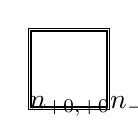
\begin{tikzpicture}
		\tikzstyle{every node}=[draw, shape=rectangle, minimum size=\nodesize cm, font=\small];
		\draw[double] (0,0) rectangle (\colsize,\rowsize);
		\nodeat{2}{1} {$n_{+0,+0}$};
		\nodeat{1}{1} {$n_{-1,+0}$};
		\nodeat{2}{2} {$n_{+0,+1}$};
	\end{tikzpicture}
	\caption{Relative structured position\label{fig:relative-structured-position}}
}
{
	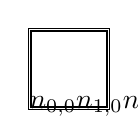
\begin{tikzpicture}
		\tikzstyle{every node}=[draw, shape=rectangle, minimum size=\nodesize cm, font=\small];
		\draw[double] (0,0) rectangle (\colsize,\rowsize);
		\nodeat{0}{0} {$n_{0,0}$};
		\nodeat{1}{0} {$n_{1,0}$};
		\nodeat{0}{1} {$n_{0,1}$};
	\end{tikzpicture}
	\caption{Absolute structured position\label{fig:absolute-structured-position}}
}
\caption{Depiction of \emph{relative} structured position versus \emph{absolute} structured position. The row and column counts are increasing down and to the right, respectively. The borders indicate structured regions, whose origin resides in the top-left corner.\label{fig:structured-position}}
\end{figure}



\section{Properties of detection algorithm}

\subsection{Eager detection}
An eager (or greedy) detection algorithm will include every structured element if finds immediately, regardless of the long term consequences. While this strategy may lead to suboptimal results, it avoids backtracking the structure detection which may be prohibitively costly.


\begin{figure}
\pgfplotstableread{
	2 2 2 2 2 2 0
	2 2 1 2 2 0 0
	0 0 1 0 0 0 0
	0 0 1 0 0 0 0
}{\eagermatrix}
\pgfplotstableread{
	2 2 2 2 2 2 0
	2 2 0 2 2 0 0
	1 1 1 1 1 1 1
	1 1 1 1 1 1 1
}{\noneagermatrix}

\sidebyside
{
	\drawmatrix[cell wd=0.6, cell ht=0.6]{\eagermatrix}
	\caption{Eager detection may greedily add the northern cell, yielding a suboptimal structured region.}
}
{
	\drawmatrix[cell wd=0.6, cell ht=0.6]{\noneagermatrix}
	\caption{A non-eager algorithm could instead decide to ignore the northern cell, yielding a larger structured region.}
}
\caption{Eager versus non-eager detection. Black cells and white cells denote unstructured and structured elements, respectively. Red cells denote structured elements detected as forming a rectangular structured region.}
\end{figure}



\subsection{Contiguous detection}
An algorithm which exhibits continuous detection always adds a structured element which is contiguous to the structured region thus far. The implication is that the relative structured position is always known. This greatly simplifies detection, as all adjacent structured elements are known at any point in time, and structured elements need not be repositioned in the structured region.

In the case of non-contiguous detection, any non-contiguous blobs need to be consolidated. These blobs may be one of three cases:
\begin{enumerate}
\item Disjoint
These may simply be taken as two separate structured regions.

\item Compatible
The blobs can be merged in a lossless manner to form a single structured region.

\item Incompatible
The blobs cannot be merged without loss of structure due to inconsistencies between the blobs. It is then necessary to discard some structured elements.
\end{enumerate}


% Contiguous versus non-contiguous
\begin{figure}
\pgfplotstableread{
	0 1 1 1 0 0 0 0 0
	0 1 1 1 1 0 0 0 0
	0 1 1 1 0 0 0 0 0
	0 0 1 0 0 0 0 0 0
	0 0 0 0 0 0 0 0 0
}{\contiguousmatrix}
\pgfplotstableread{
	0 1 1 1 0 0 0 0 0
	0 1 1 1 1 0 0 1 0
	0 1 1 1 0 0 1 1 0
	0 0 1 0 0 0 0 0 0
	0 0 0 0 0 0 0 0 0
}{\noncontiguousmatrix}

\sidebyside
{
	\drawmatrix[cell wd=0.6, cell ht=0.6]{\contiguousmatrix}
	\caption{Contiguous detection always adds cells adjacent to the structured region detected thus far.}
}
{
	\drawmatrix[cell wd=0.6, cell ht=0.6]{\noncontiguousmatrix}
	\caption{Non-contiguous detection may add cells which do not border the structured region detected thus far.}
}
\caption{Contiguous detection versus non-contiguous detection algorithms. White cells denote structured elements which have not been added to the structured region. Red cells denote structured elements detected thus far.}
\end{figure}

% Types of non-contiguous
\begin{figure}
\pgfplotstableread{
	0 1 1 1 0 0 0 0 0
	0 1 1 1 1 0 0 0 0
	0 1 1 1 0 3 3 3 0
	0 0 1 0 3 3 3 3 0
	0 0 0 0 0 3 3 0 0
}{\disjointmatrix}
\pgfplotstableread{
	0 1 1 1 0 0 0 0 0
	0 1 1 1 1 3 0 0 0
	0 1 1 1 3 3 3 3 0
	0 0 1 0 3 3 3 3 0
	0 0 0 0 0 3 3 0 0
}{\consistentmatrix}

\sidebyside
{
	\drawmatrix[cell wd=0.6, cell ht=0.6, alt color=blue]{\disjointmatrix}
	\caption{Disjoint blobs of structured elements.}
}
{
	\drawmatrix[cell wd=0.6, cell ht=0.6, alt color=blue]{\consistentmatrix}
	\caption{Consistent blobs of structured elements.}
}
\caption{Cases that may arise with non-contiguous detection.}
\end{figure}


\subsection{Post processing requirements}
Different algorithms will require different levels of post-processing in order to yield a rectangular structured region. Some may require a simple operation, such as trimming incomplete rows, while others may require more complex operations to achieve this goal.


\subsection{Detection traversal patterns}
The order in which structured elements are detected in a structured region is important; it imposes some constraints on the data structure representing it. Given the dimensions of the structured region, and knowledge of the absolute structured positions of elements as they are discovered, a simple 2D array allocation would suffice. Any detection order, as is convenient, may be used in this case. However, neither of those facts are known a priori in general.

Various detection traversals orders and their merits are discussed below.

\subsubsection{Single-row append-only}
\label{append-detection}
The structured region is grown in a constant direction, for example a single row of structured elements, appended to consecutively. This can be implemented efficiently using either a singly-linked list or a dynamic array with amortized constant time append operation.

\subsubsection{Single-row append/prepend}
\label{append-prepend-detection}
The structured region is grown in either of two directions, for example a single row of structured elements, appended and prepended to. This can be implemented efficiently using a double-ended queue with amortized constant time append and prepend operations.

\subsubsection{Row-oriented detection}
The structured region is represented as a group of rows, with the elements in individual rows grown using one of the above methods. The order in which the rows themselves are grown may also be utilize the same methods, with a nested data structure being a suitable implementation. For example, if rows are detected in an append-only fashion, and the individual elements are detected using append and prepend operations, then a suitable data structure would be a singly-linked list of double-ended queues.

\subsubsection{Indeterminate order detection}
The structured region is grown in a non-linear order: grown elements may not always be contiguous to the structured region thus far. If the growth is indeed non-contiguous, the relative structured positions are \emph{not} always known, and structured elements may need to be repositioned. A possible implementation would be a jagged 2D array, that is an array of arrays, which is expanded as needed. A flat-array-based 2D array would (in the worst case) require reallocating all elements upon expansion, as opposed to reallocating a single row in the case of a jagged 2D array.





Consider contiguity in a figure!!!!

---------------------
                    |
                    |
          A         |
        -------------
     B  | C |
        |----
        |
---------

If the the region were to be grown to include include element C, it must be the case that C is adjacent to both A and B, but is not adjacent to any other structured element thus far. Since the structure is always contiguous, we know at every point whether any two structured elements ought to be adjacent.


\section{ALGORITHMS}

\subsection{Length-first search}
We begin with the most greedy approach.
\begin{enumerate}
\item Starting from a seed vertex, grow a quad.
\item The quad is grown along one axis, both forwards and backwards, as far as possible. This forms the length of the structured region.
\item The quad row grown above is extended along the orthogonal axis, both forwards and backwards, as far as possible. This forms the width of the structured region.
\end{enumerate}

This algorithm is simple in concept and implementation. Its runtime complexity is $O(STRUCTURED VERTICES DETECTED)$, and has a constant storage requirement. The vertices can be stored as they are detected by using, for example, a double-ended queue per row.

FIGURE: BEHAVIOUR IN A GOOD ENVIORNMENT
FIGURE: BEHAVIOUR WITH BAD SEED


Two types of techniques exist: seed-based, and global based. A seed-based technique starts with a seed, and grows from there. A global-based technique starts with all the orthogonal axis

\chapter{Structure Extraction}
\newcommand{\Structured}{V_{structured}}
\newcommand{\AdjVV}{Adj_{\VertexSet\VertexSet}}
\newcommand{\vinit}{v_{init}}



\subsection{Inputs}
\begin{enumerate}
\item A non-reflexive and symmetric vertex-vertex adjacency relation:
$$ \AdjVV: \VertexSet \mapsto \powerset{\VertexSet} $$

\item A set of visited vertices
$$ \Visited \subseteq \VertexSet $$

\item An unvisited start vertex
$$ \vinit \in \VertexSet \setminus \Visited $$
\end{enumerate}


\subsection{Outputs}
\begin{enumerate}
\item A structured set of vertices $\Structured \subseteq \VertexSet \setminus \Visited $ forming the extracted structured region.
The vertices $\Structured$ are structured on a 2-dimensional Cartesian lattice with $m$ rows and $n$ columns.
\end{enumerate}


%%%% PHASE 1

%% Phase 1 summary
\subsection{Phase 1: Grow a quad}
Starting from the initial vertex $\vinit$, call it $n_{1,1}$, we would like to discover three other vertices $n_{1,2}$, $n_{2,1}$, and $n_{2,2}$ that, together with $n_{1,1}$, form a quad in a structured quad region. They must satisfy the following constraints:

\begin{itemize}
\item Each of the four vertices must have exactly 4 neighbours.
\item Each of the following pairs of vertices are neighbours: $n_{1,1}$~and~$n_{1,2}$ ; $n_{1,2}$~and~$n_{2,2}$ ; $n_{2,2}$~and~$n_{2,1}$ ; $n_{2,1}$~and~$n_{1,1}$.
\item Each of the vertices must \emph{not} neighbour any vertex that is part of the structured region thus far, apart from those vertices explicitly mentioned.
\end{itemize}

%% Phase 1 diagram

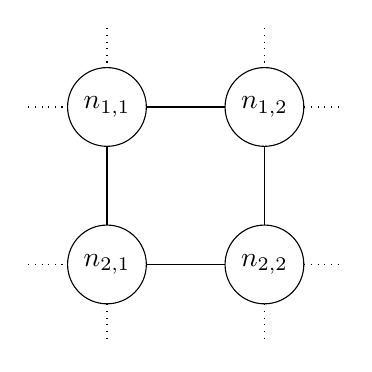
\begin{tikzpicture}[scale=1]
		% Default action for each node
		\tikzstyle{every node}=[draw, shape=circle, minimum size=1cm];

											\coordinate (northleft) at (0, 2);	\coordinate (northright) at (2, 2);
		\coordinate (westup) at (-1,1);		\node (r1c1) at (0,1) {$n_{1,1}$};	\node (r1c2) at (2,1) {$n_{1,2}$};	\coordinate (eastup) at (3,1);
		\coordinate (westdown) at (-1,-1);	\node (r2c1) at (0,-1) {$n_{2,1}$};	\node (r2c2) at (2,-1) {$n_{2,2}$};	\coordinate (eastdown) at (3,-1);
											\coordinate (southleft) at (0, -2);	\coordinate (southright) at (2, -2);

		% Horizontals
		\draw[outside] (westup) -- (r1c1);
		\draw (r1c1) -- (r1c2);
		\draw[outside] (r1c2) -- (eastup);

		\draw[outside] (westdown) -- (r2c1);
		\draw (r2c1) -- (r2c2);
		\draw[outside] (r2c2) -- (eastdown);

		% Verticals
		\draw[outside] (northleft) -- (r1c1);
		\draw (r1c1) -- (r2c1);
		\draw[outside] (r2c1) -- (southleft);

		\draw[outside] (northright) -- (r1c2);
		\draw (r1c2) -- (r2c2);
		\draw[outside] (r2c2) -- (southright);
	\end{tikzpicture}

%% Phase 1 algorithm

\subsubsection{Algorithm}

\begin{enumerate}
\item If $\vinit$ does not have exactly 4 neighbours, that is $ \card{\AdjVV(\vinit)} \neq 4 $, return immediately with $\Structured = \varnothing$.
\item Let $ n_{1,1} = \vinit $, and let $ a, b, c \in \AdjVV(\vinit) $ be distinct vertex neighbours of $\vinit$. Consider vertices $a$ and $b$. If they do not both have exactly 4 neighbours, then they cannot form a part of a structured quad region. Return immediately with $\Structured = \varnothing$.

\item Otherwise, there are three cases:

	%%%% BEGIN THREE CASES
	\begin{enumerate}[label=Case \alph*)]

	%% Straight line case
	\item $a$ and $b$ have exactly one neighbour in common, which must be $n_{1,1}$ by construction, expressed by:
	$$ \card{\AdjVV(a) \cap \AdjVV(b)} = 1$$
	$a, n_{1,1}, b $ are \emph{topologically} along a straight line of a structured grid, and hence cannot form a quad.
	We therefore consider $b$, $n_{1,1}$, and  $c$ instead as candidates, letting $n_{2,1} = b$ and $n_{1,2} = c$.
	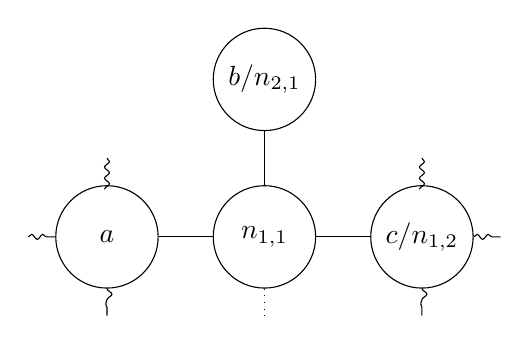
\begin{tikzpicture}
		% Default action for each node
		\tikzstyle{every node}=[draw, shape=circle, minimum size=1.3cm];

										\coordinate (northleft) at (-1,2);	\node (b) at (1,3) {$b / n_{2,1}$};	\coordinate (northright) at (3,2);
		\coordinate (west) at (-2,1);	\node (a) at (-1,1) {$a$};			\node (n11) at (1,1) {$n_{1,1}$};	\node (c) at (3,1) {$c / n_{1,2}$};	\coordinate (east) at (4,1);
										\coordinate (southleft) at (-1,0);	\coordinate (southmid) at (1,0);	\coordinate (southright) at (3,0);

		\draw[anywhere] (west) -- (a);
		\draw (a) -- (n11) -- (c);
		\draw[anywhere] (c) -- (east);

		\draw[anywhere] (northleft) -- (a) -- (southleft);
		\draw (b) -- (n11);
		\draw[outside] (n11) -- (southmid);
		\draw[anywhere] (northright) -- (c) -- (southright);
	\end{tikzpicture}


	%% Angle case
	\item $a$ and $b$ have exactly two neighbours in common, one of which must be $n_{1,1}$ by construction, expressed by:
	$$ \card{\AdjVV(a) \cap \AdjVV(b)} = 2$$
	We continue with vertices $a$, $n_{1,1}$, and $b$ as candidates, letting $n_{2,1} = a$ and $n_{1,2} = b$.
	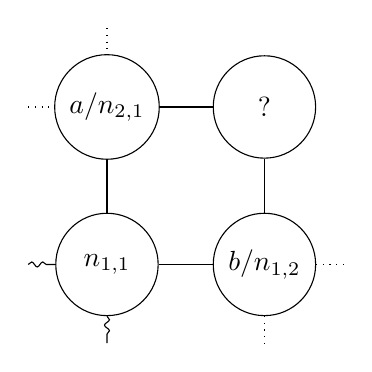
\begin{tikzpicture}
		% Default action for each node
		\tikzstyle{every node}=[draw, shape=circle, minimum size=1.3cm];

											\coordinate (northleft) at (-1,4);		\coordinate (northright) at (1,4);
		\coordinate (westup) at (-2,3);		\node (a) at (-1,3) {$a / n_{2,1}$};	\node (d) at (1,3) {$?$};			\coordinate (eastup) at (2,3);
		\coordinate (westdown) at (-2,1);	\node (n11) at (-1,1) {$n_{1,1}$};		\node (b) at (1,1) {$b / n_{1,2}$};	\coordinate (eastdown) at (2,1);
											\coordinate (southleft) at (-1,0);		\coordinate (southright) at (1,0);



		\draw[outside] (westup) -- (a);
		\draw (a) -- (d);
		% \draw (d) -- (eastup);

		\draw[anywhere] (westdown) -- (n11);
		\draw (n11) -- (b);
		\draw[outside] (b) -- (eastdown);

		\draw[outside] (northleft) -- (a);
		\draw (a) -- (n11);
		\draw[anywhere] (n11) -- (southleft);

		% \draw (northright) -- (d);
		\draw (d) -- (b);
		\draw[outside] (b) -- (southright);

	\end{tikzpicture}


	\item $a$ and $b$ have more than two neighbours in common\footnote{note that the set is non-empty by construction}, expressed by:
	$$ \card{\AdjVV(a) \cap \AdjVV(b)} > 2$$
	We cannot form a quad, and hence return immediately with $\Structured = \varnothing$.

	\end{enumerate}
	%%%% END THREE CASES

\item Find the common neighbours of $n_{2,1}$ and $n_{1,2}$. If there are not exactly two neighbours, return immediately with $\Structured = \varnothing$.

\item One of the two neighbours must be $n_{1,1}$ by construction. Let the other neighbour be $n_{2,2}$

\item Let $N = \{ n_{1,1}, n_{1,2}, n_{2,1}, n_{2,2} \}$. If any vertex $n \in N$ is in $\Visited$, that is $N \cap \Visited \neq \varnothing$, then return immediately with $\Structured = \varnothing$. Otherwise add the vertices in $N$ to $\Visited$.

\item Ensure for every vertex $n \in N$ that its visited neighbours, $\AdjVV(n) \cap \Visited$, are exactly those explicitly stated above. If this is not the case, remove $N$ from $\Visited$ and return immediately with $\Structured = \varnothing$.

\item Set $\Structured = \{ n_{1,1}, n_{1,2}, n_{2,1}, n_{2,2} \}$, and continue to the next phase.

The structured region looks as follows thus far.
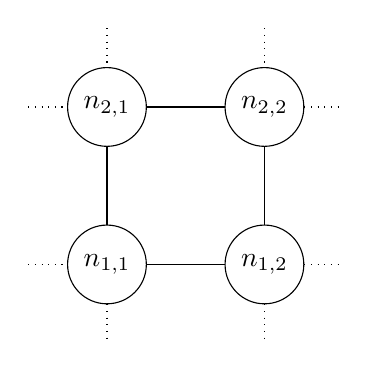
\begin{tikzpicture}
	% Default action for each node
	\tikzstyle{every node}=[draw, shape=circle, minimum size=1cm];

										\coordinate (northleft) at (-1,4);	\coordinate (northright) at (1,4);
	\coordinate (westup) at (-2,3);		\node (n21) at (-1,3) {$n_{2,1}$};	\node (n22) at (1,3) {$n_{2,2}$};	\coordinate (eastup) at (2,3);
	\coordinate (westdown) at (-2,1);	\node (n11) at (-1,1) {$n_{1,1}$};	\node (n12) at (1,1) {$n_{1,2}$};	\coordinate (eastdown) at (2,1);
										\coordinate (southleft) at (-1,0);	\coordinate (southright) at (1,0);



	\draw[outside] (westup) -- (n21);
	\draw (n21) -- (n22);
	\draw[outside] (n22) -- (eastup);

	\draw[outside] (westdown) -- (n11);
	\draw (n11) -- (n12);
	\draw[outside] (n12) -- (eastdown);

	\draw[outside] (northleft) -- (n21);
	\draw (n21) -- (n11);
	\draw[outside] (n11) -- (southleft);

	\draw[outside] (northright) -- (n22);
	\draw (n22) -- (n12);
	\draw[outside] (n12) -- (southright);

\end{tikzpicture}

\end{enumerate}



\chapter{Future works}
This project covered extensive grounds on BLA BLA BLA BLA. With that said, there are plenty of interesting future directions to be pursued, and intriguing tangents to be followed.

\section{Triangular and non-quad meshes}
%% TODO cross reference: In section XXX we claim/discuss how..
Our algorithms are designed to work on meshes with exclusively quadrilateral faces. It is not difficult to imagine modifying the structure detection algorithms to find quadrilateral structure in meshes containing mixed face types such as triangles and hexagons. What would be

We claim that our detection approach can encompass triangle-based structure, and in general any repeating pattern of vertices which may be inscribed in a quadrilateral.


\section{Different types of structure}
Radial, hierarchical
c.f. what I say about polar coordinates
reference hierarchical adaptive mesh refinement, etc

\section{3D meshes}
From surface to volume, in THREE DEE

Could we detect any pattern inscribable in a cube?

\section{Investigate structure growth strategies}
Try the various rectangle growth strategies we outlined.
Try non-rectangular structured regions.
Try different completely techniques (e.g. particle shooting)

Reference particle shooting

\section{Parallelized detection}
That is, detect regions in parallel. Discuss merging regions

Reference particle shooting?


\section{Parallel implementation}
How should we detect and use regions suited for parallel computation?
Likely that we detect the maximum region possible, and then break it down into parts.

Reference the many parallel papers.


\section{Adaptive runtime detection}
Could the detection be performed during runtime, in parallel say. We can hotswap in the structured regions incrementally between iterations as they are detected

Reference the parallel adaptive mesh refinement paper

\section{Geometry based detection}
Could we exploit the underlying geometry to aid in detecting structure?
c.f. Italian paper




\nocite{*} % Show all Bib-entries
\bibliographystyle{plainurl}
\bibliography{thesis}

\end{document}
